\PassOptionsToPackage{cmyk, hyperref, dvipsnames}{xcolor}
\PassOptionsToPackage{x-4}{pdfx}  % X is printing standard. 5g is the latest supported version.
\documentclass[fontsize=10pt, paper=a5, final]{scrbook} % KOMA-Script book

%\usepackage[cmyk, hyperref, dvipsnames]{xcolor} %The two first options are for pdf-x 
\usepackage[x-4]{pdfx} % X is printing standard. 5g is the latest supported version.

\usepackage{fontspec}


\usepackage{microtype}
\pagestyle{empty}
\raggedright
\usepackage[hyphenation,lastparline,nosingleletter]{impnattypo} %draft
\frenchspacing   % Do not include extra space after sentences.

\usepackage{xpatch} %Adjust the spacing in smallcaps
\xapptocmd{\scshape}{\spaceskip=2\fontdimen2\font plus 2\fontdimen3\font minus \fontdimen4\font	\xspaceskip=0\fontdimen7\font}{}{}

\usepackage[spanish,british]{babel}

\usepackage{graphicx}
\usepackage{tikz}
\usetikzlibrary{calc,shapes,positioning}

\usepackage[outer=0mm, inner=0mm, top=0mm, bottom=0mm]{geometry}
\usepackage{placeins}

\usepackage{ccicons}

\frenchspacing   % Do not include extra space after sentences.

\usepackage{enumitem}
\setlist{leftmargin=0mm}% Remove indentation in bulletpoints
%\setlist[itemize]{before=\csname par\endcsname\raggedright,	partopsep=0pt}
\setlist[itemize]{partopsep=0pt}


\def\helplines{0}

\setmainfont{tex-gyre-pagella}


%ebgaramond
%Cardo
\newcommand{\english}[1]{\fontspec{imfellenglish} \large \color{Maroon} #1}
\newcommand{\spanish}[1]{\begin{otherlanguage}{spanish}
	\fontspec{IbarraReal} \large \color{RoyalBlue} #1
\end{otherlanguage}}

\newcommand{\sketchpage}[1]{\begin{figure}
	\includegraphics[width=\pagewidth]{sketches/#1.pdf}
\end{figure}}

\newcommand{\doindent}{\hspace{1em}}
\newcommand{\N}{0.995}

\hyphenation{de-ac-ti-va-tes}

\begin{document}

\begin{center}

\begin{tikzpicture}
    \begin{scope}[x={(current page.south east)},y={(current page.north west)}]
        \node[anchor=south west,inner sep=0, draw] (image)  at (0.35, 0.3) {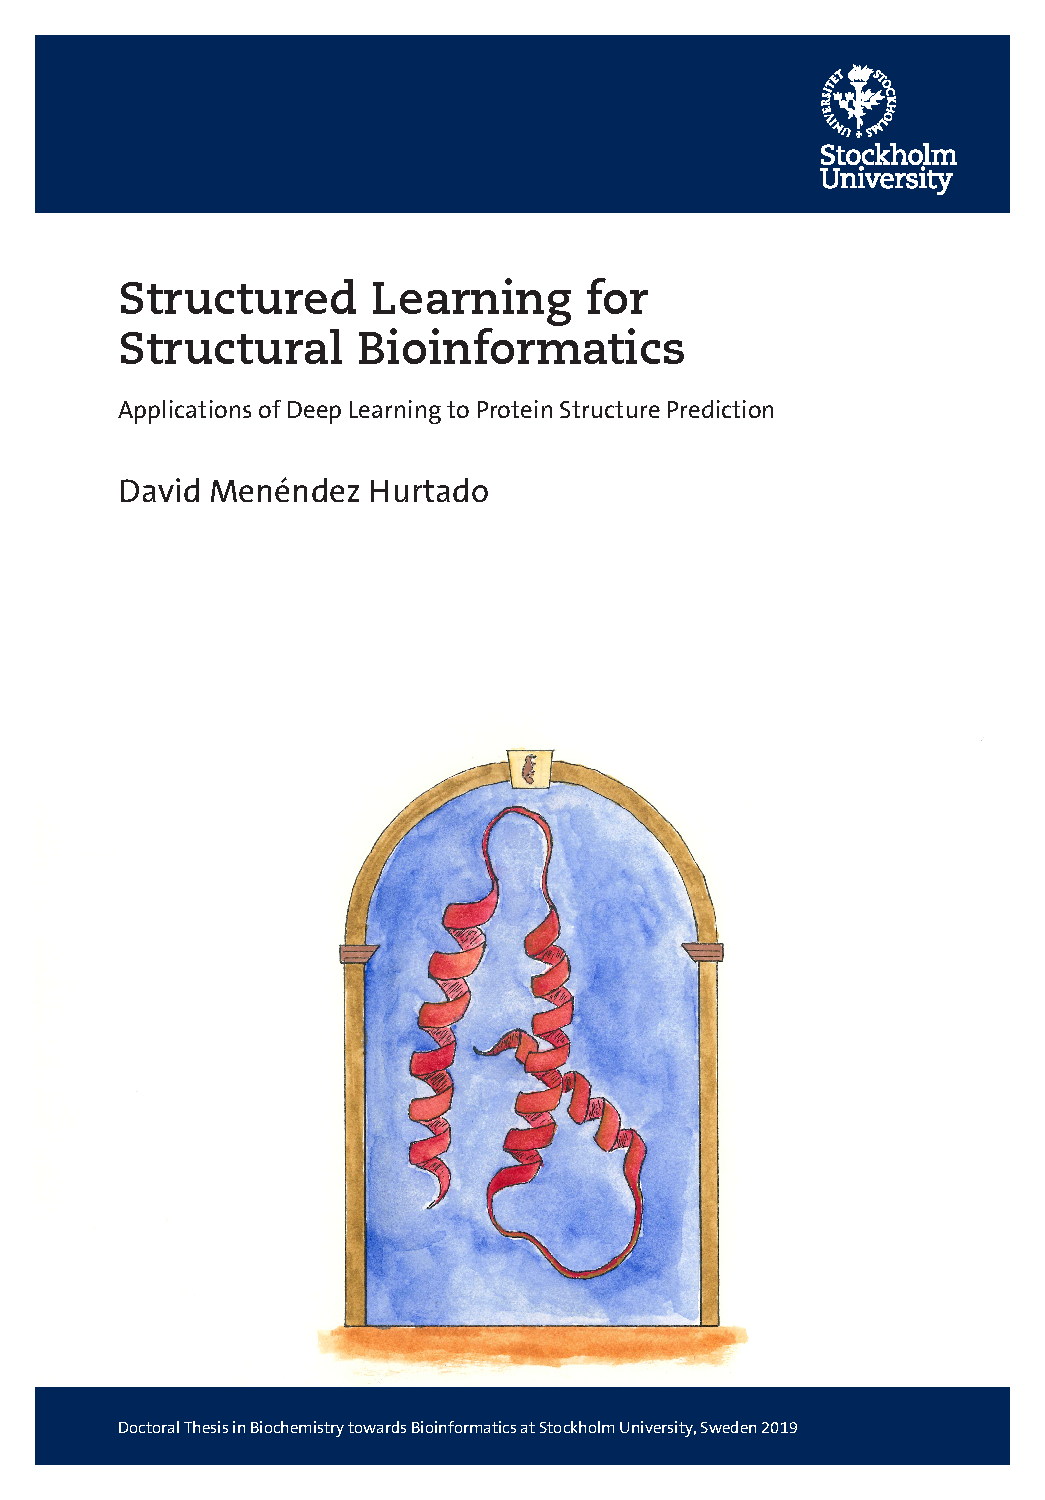
\includegraphics[height=0.6\pageheight]{scans/cover.pdf}};
    	\if\helplines1
        	\draw[help lines,xstep=.1,ystep=.1] (0,0) grid (\N,\N);
        \fi
        \if\helplines0
        	\path[help lines,xstep=.1,ystep=.1] (0,0) grid (\N,\N);
        \fi
        
        \node[align=left, anchor=west] (en) at (0.1, 0.1) {\english{\Huge A visual introduction to my thesis.}};
        \node[align=left, anchor=west] (es) at (0.1, 0.2)  {\spanish{\Huge Una introducción visual a mi tesis.}};
        
    \end{scope}
\end{tikzpicture}
\end{center}


% % image done
% %--- image missing
%
%


\newgeometry{margin=1in, bottom=2in}
\phantom{x}

\vfill
David Menéndez Hurtado

\emph{\footnotesize This work is licensed under a Creative Commons Attribution 4.0 International License.}
\ccby


\phantom{x}

Technical review: Arne Elofsson

Revisión de la traducción: Ana d'Ors

\phantom{x}

Artwork in ink and watercolours.



\restoregeometry
\newpage
\begin{center}
\begin{tikzpicture}
    \begin{scope}[x={(current page.south east)},y={(current page.north west)}]
        \if\helplines1
        	\draw[help lines,xstep=.1,ystep=.1] (0,0) grid (\N, \N);
        \else
            \path[help lines,xstep=.1,ystep=.1] (0,0) grid (\N, \N);
        \fi
        \node[text width=0.4\pagewidth, align=center, anchor=north west](titleen) at (0.075, 0.7){\english{\Huge  Introduction}};
		\node[text width=0.4\pagewidth, align=justify, below=1cm of titleen] {\english{This is an attempt to explain my thesis in a way that is accessible for everyone.
		
		\doindent The comic, just as the thesis, is structured in the following way:
		
		\begin{itemize}
		\item First, some background. I will explain what proteins are, why we care, and the problems I worked on.
		\item Then, the papers I published during my PhD. Brief summary of the content, and what I think is the most important message from each.
		\end{itemize}}};
		
		
		\node[text width=0.4\pagewidth, align=center, anchor=north west] (titlees) at (0.525, 0.72) {\spanish{\Huge Introdución}};
		\node[text width=0.4\pagewidth, align=justify, below =1cm of titlees] {\spanish{Este comic es un intento de explicar mi tesis de una forma accessible a todos.
		
		\doindent Al igual que la tesis que acompaña, el comic está dividido en dos partes:
		
		\begin{itemize}
		\item Primero, algo información básica. Explicaré qué son las proteínas y por qué nos importan, además de presentar los problemas en los que trabajé.
		\item Después, los artículos publicados. Un breve resumen de cada uno, explicando lo que, en mi opinión, es el mensaje más importante de cada uno.
		\end{itemize}}};
    \end{scope}

\end{tikzpicture}
\end{center}


\begin{center}
\begin{tikzpicture}
    \node[anchor=south west,inner sep=0] (image)  at (0,0) {\includegraphics[trim={2mm, 2mm, 2mm, 2mm}, width=0.995\pagewidth]{scans/pan-3.pdf}};
    
   
    \begin{scope}[x={(image.south east)},y={(image.north west)}]
        \if\helplines1
        	\draw[help lines,xstep=.1,ystep=.1] (0,0) grid (1,1);
        \fi
        %\node(title) at (0.5, 0.9) {\Huge {Proteins as machines}};
        \node[align=center, anchor=north, text width=0.4\pagewidth](en) at (0.67, 0.815) {\english{\Large Proteins are the fundamental machines of the cell, and at the same time, the workers that direct them.}};
        \node[align=center, anchor=north, text width=0.3\pagewidth](es) at (0.27, 0.55) {\spanish{ \Large Las proteínas son las maquinaria fundamental de las células, y al mismo tiempo, los obreros que las accionan.}};
    \end{scope}

\end{tikzpicture}
\end{center} %
\begin{center}
\begin{tikzpicture}
    \node[anchor=south west,inner sep=0] (image)  at (0,0) {\includegraphics[trim={2mm, 2mm, 2mm, 2mm},width=0.995\pagewidth]{scans/panel-5.pdf}};
    
    
    \begin{scope}[x={(image.south east)},y={(image.north west)}]
        \if\helplines1
        	\draw[help lines,xstep=.1,ystep=.1] (0,0) grid (\N,\N);
        \else
        	\path[help lines,xstep=.1,ystep=.1] (0,0) grid (\N,\N);
        \fi
        \node[align=center, anchor=north, text width=0.3\paperwidth](en1) at (0.5, 0.95) {\english{They perform a variety of tasks, from sending signals to other cells}};
        
        \node[align=center, anchor=north, text width=0.3\paperwidth, below=3mm of en1] {\spanish{Realizan una gran variedad de funciones, desde transmitir señales }};
        
        % %
        \node[align=center, anchor=north, text width=0.3\paperwidth] at (0.2, 0.4) {\english{to pumping water and substances in and out of the cell.}};
        
        \node[align=center, anchor=north, text width=0.3\paperwidth] at (0.8, 0.4) {\spanish{a bombear agua y substancias dentro y fuera de la célula.}};
               
    \end{scope}
    
\end{tikzpicture}
\end{center}

 %
%
\begin{center}
	\begin{tikzpicture}
	\node[anchor=south west,inner sep=0] (image)  at (0,0) {\includegraphics[trim={2mm, 2mm, 2mm, 2mm}, clip, angle=180, width=0.995\pagewidth]{scans/pan-5.pdf}};
	
	
	\begin{scope}[x={(image.south east)},y={(image.north west)}]
	\if\helplines1
	\draw[help lines,xstep=.1,ystep=.1] (0,0) grid (1,1);
	\fi

	\node[align=center, anchor=south west, text width=0.3\pagewidth](en) at (0.05, 0.62) {\english{Understanding proteins help us understand how the machines break - what we call disease - and how to fix it, ie., heal.}};
	\node[align=center, anchor=north west, text width=0.4\pagewidth](es) at (0.55, 0.48) {\spanish{Entender cómo funcionan las proteínas nos ayuda a entender cómo y por qué estas máquinas se estropean - lo que llamamos enfermedad - y cómo arreglarlas, es decir, curar.}};
	\end{scope}
	
	\end{tikzpicture}
\end{center} %
\begin{center}
\begin{tikzpicture}
    \node[anchor=south west,inner sep=0] (image)  at (0,0) {\includegraphics[trim={2mm, 2mm, 2mm, 2mm},width=0.995\pagewidth]{scans/panel-9.pdf}};
    
    
    \begin{scope}[x={(image.south east)},y={(image.north west)}]
        \if\helplines1
        	\draw[help lines,xstep=.1,ystep=.1] (0,0) grid (1,1);
        \fi
        \node[align=justify, anchor=north west, text width=6cm](en) at (0.5, 0.9) {\english{We can also block, divert, or reinforce the signals using chemical substances, that we call drugs.
        
        \doindent For example, Naproxen deactivates a protein whose taks is to send the signal of pain.}};
        
        \node[align=justify, anchor=north west, text width=6cm](es) at (0.1, 0.2) {\spanish{También podemos bloquear, redirigir, o reforzar estas señales usando substancias químicas: lo que llamamos medicinas.}
        
        \spanish{\doindent Por ejemplo, el Naproxeno desactiva una proteína encargada de transmitir el dolor.}};
    \end{scope}
    
\end{tikzpicture}
\end{center} %
%
\begin{center}
\begin{tikzpicture}
    \node[anchor=south west,inner sep=0] (image)  at (0,0) {\includegraphics[trim={2mm, 2mm, 2mm, 2mm}, width=0.995\pagewidth]{scans/201909201655.pdf}};
    
   
    \begin{scope}[x={(image.south east)},y={(image.north west)}]
        \if\helplines1
        	\draw[help lines,xstep=.1,ystep=.1] (0,0) grid (1,1);
        \fi
        \node[align=justify, anchor=north west, text width=0.6\pagewidth] at (0.3, 0.95) {\english{Proteins are long chains of individual blocks called amino acids.}};
        \node[align=justify, anchor=north west, text width=0.3\pagewidth] at (0.65, 0.67) {\english{They are all almost identical, except for the branches: the \emph{side-chains}.}};
         \node[align=justify, anchor=north west, text width=0.35\pagewidth] at (0.55, 0.50) {\english{These long chains fold unto themselves, forming complicated structures. The protein is born and it is thus, ready to perform its specific function.}};
         \node[align=center, anchor=north, text width=0.4\pagewidth] at (0.3, 0.09) {\english{We want to know how to get from the sequence of amino acids to the 3D structure.}};
         
         % % % %
        \node[align=left, anchor=north west, text width=0.5\pagewidth] at (0.45, 0.85) {\spanish{Las proteínas son largas cadenas cuyos eslabones se llaman aminoácidos.}};
        
        \node[align=justify, anchor=north west, text width=0.3\pagewidth] at (0.1, 0.7) {\spanish{Son todos casi idénticos, excepto por las ramas: las \emph{cadenas laterales}.}};
        
        \node[align=justify, anchor=north west, text width=0.3\pagewidth] at (0.04, 0.60) {\spanish{Cuando estas cadenas se pliegan sobre sí mismas en estructuras complicadas, tenemos una proteína capaz de realizar una función concreta.}};
        
        \node[align=center, anchor=north , text width=0.4\pagewidth] at (0.7, 0.09) {\spanish{Queremos saber cómo ir de la secuencia de aminoácidos a esta estructura en \oldstylenums{3}\textsc{d}.}};
        
    \end{scope}

\end{tikzpicture}
\end{center} %
\begin{center}
\begin{tikzpicture}
    \node[anchor=south west,inner sep=0] (image)  at (0,0) {\includegraphics[trim={2mm, 2mm, 2mm, 2mm},width=0.995\pagewidth]{scans/panel-2.pdf}};
    
    
    \begin{scope}[x={(image.south east)},y={(image.north west)}]
        \if\helplines1
        	\draw[help lines,xstep=.1,ystep=.1] (0,0) grid (1,1);
        \fi
        \node[align=center, text width=0.4\pagewidth,anchor=north](en) at (0.7, 0.9) {\english{Excuse me, but why would we care about any of this?
        
        \footnotesize{Will it be on the exam?}}};
        \node[align=center, text width=0.4\pagewidth, anchor=north](es) at (0.21, 0.85) {\spanish{Perdón, pero... ¿por qué nos debe importar nada de esto?
        
        \footnotesize{¿Entra en el examen?}}};
    \end{scope}
    
\end{tikzpicture}
\end{center} %
%
\begin{center}
\begin{tikzpicture}
    \node[anchor=south west,inner sep=0] (image)  at (0,0) {\includegraphics[trim={2mm, 2mm, 2mm, 2mm},width=0.995\pagewidth]{scans/pg_0001.pdf}};
    
    
    \begin{scope}[x={(image.south east)},y={(image.north west)}]
        \if\helplines1
        	\draw[help lines,xstep=.1,ystep=.1] (0,0) grid (1,1);
        \fi
        \node[align=justify, text width=0.4\pagewidth](en) at (0.7, 0.85) {\english{Performing an experiment to obtain the sequence of amino acids that form a protein is easy and straightforward.
        
        \doindent Nowadays, sequencing all the proteins of a human - a tad under hundred thousand - costs less than 1\,000 €.}};
        \node[align=justify, anchor=north west, text width=0.4\pagewidth](es) at (0.1, 0.3) {\spanish{Realizar el experimento para obtener la secuencia de aminoácidos que forman la proteína es fácil y sencillo.
        
        
        \doindent Hoy en día, secuenciar todas las proteínas de un humano - casi cien mil - cuesta menos de \oldstylenums{1\,000} €.}};
    \end{scope}
    
\end{tikzpicture}
\end{center} %
\begin{center}
\begin{tikzpicture}
    \node[anchor=south west,inner sep=0] (image)  at (0,0) {\includegraphics[trim={2mm, 2mm, 2mm, 2mm}, width=0.995\pagewidth]{scans/pg_0004.pdf}};
    
    \begin{scope}[x={(image.south east)},y={(image.north west)}]
        \if\helplines1
        	\draw[help lines,xstep=.1,ystep=.1] (0,0) grid (1,1);
        \fi
        \node[align=justify, anchor=north west, text width=0.35\pagewidth] at (0.55, 0.9) {\english{But the path to obtain a three-dimensional structure is long and tortuous, and often fails.
        
        \vspace{1em}
        
        \doindent Obtaining the structure of a single human protein can cost several millions.
        }};
        
        \node[align=justify, anchor=north west, text width=0.35\pagewidth] at (0.05, 0.6){\spanish{Pero el proceso para obtener la estructura tridimensional es largo, tortuoso y repleto de fallos.
        
        \vspace{1em}
        
        \doindent Obtener la estructura de una sóla proteína humana puede costar millones.
        }};
    \end{scope}

\end{tikzpicture}
\end{center} %
%

\begin{center}
\begin{tikzpicture}
    \node[anchor=south west,inner sep=0] (image)  at (0,0) {\includegraphics[trim={2mm, 2mm, 2mm, 2mm}, width=0.995\pagewidth]{scans/pg_0006.pdf}};

    \begin{scope}[x={(image.south east)},y={(image.north west)}]
        \if\helplines1
        	\draw[help lines,xstep=.1,ystep=.1] (0,0) grid (1,1);
        \fi
        \node[align=center, anchor=north](0) at (0.5, 0.15) {\english{\Large But, how does a computer know how to fold proteins?}};
        
        \node[align=center, anchor=north](0) at (0.5, 0.09) {\spanish{\Large Pero, ¿cómo sabe el ordenador cómo plegar proteínas?}};
    \end{scope}

\end{tikzpicture}
\end{center} %
\begin{center}
\begin{tikzpicture}
    \node[anchor=south west,inner sep=0] (image)  at (0,0) {\includegraphics[trim={2mm, 2mm, 2mm, 2mm}, width=0.995\pagewidth]{scans/pan-4.pdf}};
    
   
    \begin{scope}[x={(image.south east)},y={(image.north west)}]
        \if\helplines1
        	\draw[help lines,xstep=.1,ystep=.1] (0,0) grid (1,1);
        \fi

        \node[align=justify, anchor=north west, text width=0.4\pagewidth](en) at (0.54, 0.95) {\english{One option is \emph{ab-initio}: starting from scratch, try a lot of different configurations, until one seems to match.}};
        
        \node[align=justify, anchor=north west, text width=0.55\pagewidth](en) at (0.38, 0.45) {\english{The other option is \emph{homology}, where the computer uses pieces from other proteins similar in sequence, for which we have the structure. Like pieces of a puzzle.}};
        
        % % %
        
        \node[align=justify, anchor=north west, text width=0.30\pagewidth](es) at (0.65, 0.8) {\spanish{Una opción es \emph{ab-initio}: empezando de cero, probando muchas configuraciones diferentes, hasta que alguna parezca coincidir.}};
        
    
        \node[align=justify, anchor=north west, text width=0.27\pagewidth](es) at (0.65, 0.35) {\spanish{La otra opción es \emph{por homología}: donde el ordenador busca en la base de datos de estructuras de proteínas por algunas similares a la nuestra, y los usa como piezas de puzle.}};
    \end{scope}

\end{tikzpicture}
\end{center} %
%
\begin{center}
\begin{tikzpicture}
    \node[anchor=south west,inner sep=0] (image)  at (0,0) {\includegraphics[trim={2mm, 2mm, 2mm, 2mm}, width=0.995\pagewidth]{scans/pg_0005.pdf}};


    \begin{scope}[x={(image.south east)},y={(image.north west)}]
        \if\helplines1
        	\draw[help lines,xstep=.1,ystep=.1] (0,0) grid (1,1);
        \fi
        \node[align=justify, anchor=north west, text width = 0.32\pagewidth](0) at (0.6, 0.9) {\english{Proteins are tightly packed inside, so when, for whatever reason, an amino acid is mutated,}};
        
        \node[align=justify, anchor=north west, text width = 0.4\pagewidth](0) at (0.52, 0.4) {\english{likely other amino acids close in space will also change to preserve the chemical properties.
        
        \doindent The amino acids that “touch" each other are called \emph{contacts}.}};
        
        % % % % % % % % % % % % %
        \node[align=justify, anchor=north west, text width = 0.32\pagewidth](0) at (0.6, 0.76) {\spanish{Las proteínas están empaquetadas muy densamente, así que cuando, por cualquier razón, un aminoácido muta,}};
        \node[align=justify, anchor=north west, text width = 0.4\pagewidth](0) at (0.52, 0.2) {\spanish{es probable que otros aminoácidos cercanos en el espacio también cambien, para preservar las propiedades energéticas.
                
        \doindent Los aminoácidos que <<se tocan>> se llaman \emph{contactos}.}};
        
        
    \end{scope}

\end{tikzpicture}
\end{center} %
\begin{center}
\begin{tikzpicture}
    \node[anchor=south west,inner sep=0] (image)  at (0,0) {\includegraphics[trim={2mm, 2mm, 2mm, 2mm}, width=0.995\pagewidth]{scans/pg_0003.pdf}};

    \begin{scope}[x={(image.south east)},y={(image.north west)}]
        \if\helplines1
        	\draw[help lines,xstep=.1,ystep=.1] (0,0) grid (1,1);
        \fi
        \node[align=justify, anchor=north west, text width = 0.36\pagewidth](0) at (0.57, 0.95) {\english{If we search for similar proteins in our databases of sequences and align them by similarity, we find that when a column - that is, a position - changes, usually other columns change as well.
        This is how we can predict contacts.}};
        
        \node[align=justify, anchor=north west, text width = 0.36\pagewidth](0) at (0.57, 0.73) {\spanish{Si buscamos proteínas similares en nuestras bases de datos de secuencias y las alineamos por similitud, encontraremos que cuando una columna - es decir, una posición - cambia, normalmente otras cambian también.
        Así es como podemos predecir contactos.}};
        
        \draw[fill=white, opacity=0.4] (0.125,0.08) -- (0.465,0.08) -- (0.46,0.448) -- (0.125, 0.45) -- cycle;
        \draw[fill=white, opacity=0.4] (0.538,0.08) -- (0.87,0.08) -- (0.87,0.448) -- (0.538, 0.45) -- cycle;
        \node[align=justify, anchor=north west, text width=0.28\pagewidth] at (0.15, 0.40)
        {\english{Technical note: if green is in contact with blue, and blue is in contact with orange, we will see a correlation between blue and orange. Distinguishing the true correlations from the spurious ones is the core of my research.}};
        
        \node[align=justify, anchor=north west, text width=0.28\pagewidth] at (0.55, 0.40)
        {\spanish{Nota técnica: si verde está en contacto con azul, y azul está en contacto con naranja, veremos una correlación entre azul y naranja. Distinguir entre las correlaciones verdaderas y espúrias es el eje de mi investigación.}};
    \end{scope}

\end{tikzpicture}
\end{center} %
%

\begin{center}
\begin{tikzpicture}
	\node[anchor=south west,inner sep=0] (image)  at (0,0) {\includegraphics[trim={2mm, 2mm, 2mm, 2mm}, width=0.995\pagewidth]{scans/pan-2.pdf}};
    \begin{scope}[x={(image.south east)},y={(image.north west)}]
		\if\helplines1
			\draw[help lines,xstep=.1,ystep=.1] (0,0) grid (1,1);
		\else
			\path[help lines,xstep=.1,ystep=.1] (0,0) grid (1,1);
		\fi
		\node[text width=0.34\pagewidth, align=justify, anchor=north east] at (1-0.03, 0.95) {\english{The last step is evaluating the quality of the models. We try to teach a computer to do this by showing it many models, good and bad, and asking it to learn the differences. This is called \emph{machine learning}.}};
		
		\node[text width=0.32\pagewidth, align=justify, anchor=north east] at (1-0.06, 0.28) {\spanish{El último paso es evaluar la calidad de los modelos. Intentamos enseñar al ordenador a hacerlo por nosotros mostrándole modelos, buenos y malos, y pidiéndole que aprenda las diferencias. Se llama \emph{aprendizaje automático}.}};
    \end{scope}

\end{tikzpicture}
\end{center}
 % ----
\begin{center}
\begin{tikzpicture}
	\node[anchor=south west,inner sep=0] (image)  at (0,0) {\includegraphics[trim={2mm, 2mm, 2mm, 2mm}, width=0.995\pagewidth]{scans/pan-1.pdf}};
    \begin{scope}[x={(image.south east)},y={(image.north west)}]
		\if\helplines1
			\draw[help lines,xstep=.1,ystep=.1] (0,0) grid (1,1);
		\else
			\path[help lines,xstep=.1,ystep=.1] (0,0) grid (1,1);
		\fi
		\node[text width=0.4\pagewidth, align=justify, anchor=north west] at (0.075, 0.92) {\english{In the later years there has been a revolution of \emph{deep learning}, a machine learning method where the computer looks at small bits, looks how they combine with each other in a hierarchical manner.}};
		
		\node[text width=0.4\pagewidth, align=justify, anchor=north west] at (0.075 * 1.75 + 0.4, 0.92) {\spanish{En los últimos años, el \emph{aprendizaje profundo} ha traído una revolución en este campo. En este sistema, el ordenador se fija en trozos pequeños, y en cómo se van combinando entre sí de forma jerárquica.}};
		
				
		\node(a) at (0.3, 0.47) {\english{\normalsize \emph{peak of inflated expectations}}};
		\node[below=4mm of a] {\spanish{\normalsize  \emph{pico de expectativas sobredimensionadas}}};
		
		\node[anchor=east](b) at (0.425, 0.21){\english{\normalsize \emph{abyss of disapointment}}};
		\node[right=6mm of b] {\spanish{\normalsize  \emph{ abismo de desilusión}}};
		
		\node(c) at (0.708, 0.385){\english{\normalsize \emph{plateau of productivity}}};
		\node[below=4mm of c]{\spanish{\normalsize \emph{meseta de productividad}}};
		
		\node[align=center, text width=0.8\paperwidth] at (0.5, 0.15) {\english{Gartner curve measures the cycle of hype of any new technology. Where are we in with deep learning?}};
		\node[align=center, text width=0.8\paperwidth] at (0.5, 0.07) {\spanish{La curva de Gartner mide el ciclo de sobreexcitación de las nuevas tecnologías. ¿Dónde estamos ahora con aprendizaje profundo?}};
    \end{scope}

\end{tikzpicture}
\end{center}
 % ----

%

\begin{center}
\begin{tikzpicture}
    \begin{scope}[x={(current page.south east)},y={(current page.north west)}]
        \if\helplines1
        	\draw[help lines,xstep=.1,ystep=.1] (0,0) grid (\N, \N);
        \else
            \path[help lines,xstep=.1,ystep=.1] (0,0) grid (\N, \N);
        \fi
        \node[text width=0.4\pagewidth, align=center, anchor=north west](titleen) at (0.075, 0.7) {\english{\Huge The papers}};
		\node[text width=0.4\pagewidth, align=justify, anchor=north west] at (0.075, 0.6) {\english{In this section I will try to summarise the highlights of the papers included in my thesis, from I to V.}};
		
		
		\node[text width=0.4\pagewidth, align=center, anchor=north west] (titlees) at (0.525, 0.4) {\spanish{\Huge Los artículos}};
		\node[text width=0.4\pagewidth, align=justify, anchor=north west] at (0.525, 0.3) {\spanish{En esta sección, intentaré resumir los aspectos más interesantes de los artículos incluídos en mi tesis, del I al V.}};
    \end{scope}

\end{tikzpicture}
\end{center}
 %
\begin{center}
\begin{tikzpicture}
    \node[anchor=south west,inner sep=0] (image)  at (0,0) {\includegraphics[trim={2mm, 2mm, 2mm, 2mm}, width=0.995\pagewidth]{scans/pg_0007.pdf}};
    
   
    \begin{scope}[x={(image.south east)},y={(image.north west)}]
        \if\helplines1
        	\draw[help lines,xstep=.1,ystep=.1] (0,0) grid (1,1);
        \fi
        \node(title) at (0.5, 0.9) {\Huge {\color{Maroon}I} - ProQ3D};
        \node[align=justify, anchor= west, text width=0.27\pagewidth](en) at (0.04, 0.4) {\english{ProQ3 is a program that tries to predict how good a protein model is.
        		In this paper, we combined the old data with a modern deep learning algorithm in a computer equipped with a GPU.
        		
        		\doindent The result, a “deep” version of ProQ3: ProQ3D.}};
        		
        \node[align=justify, anchor= west, text width=0.28\pagewidth](es) at (0.65, 0.4) {\spanish{ProQ3 es un programa que intenta predecir cómo de preciso es un modelo de una proteína.
        En este artículo, combinamos los datos antiguos con un algoritmo más moderno basado en aprendizaje profundo en un ordenador equipado con una tarjeta gráfica.
        
        \doindent El resultado, una versión <<profunda>> (\emph{\textcolor{Maroon}{“deep”}} en inglés) de ProQ3: ProQ3D.}};
    \end{scope}

\end{tikzpicture}
\end{center} %
%
\begin{center}
\begin{tikzpicture}
	\node[anchor=south west,inner sep=0] (image)  at (0,0) {\includegraphics[trim={2mm, 2mm, 2mm, 2mm}, width=0.985\pagewidth]{scans/panel-8.pdf}};
    \begin{scope}[x={(current page.south east)},y={(current page.north west)}]
		\if\helplines1
			\draw[help lines,xstep=.1,ystep=.1] (0,0) grid (\N, \N);
		\else
			\path[help lines,xstep=.1,ystep=.1] (0,0) grid (\N, \N);
		\fi
		\node(title) at (0.5, 0.9) {\Huge {\color{Maroon}II} - PconsFold2};
		
		\node[align=center](a) at (0.5, 0.85) {\english{In this paper, we built a pipeline for protein \emph{ab initio} structure prediction.}};
		
		\node[anchor=north](b) at (0.7, 0.76) {\english{From the sequence...}};
		\node[anchor=south](c) at (0.25, 0.6) {\english{...we predict the contacts...}};
		\node[anchor=north](d) at (0.70, 0.44) {\english{...use them to build a pool of models...}};
		\node[anchor=north](e) at (0.25, 0.15) {\english{...and we pick the best ones.}};

		\node[align=center, text width=0.9\pagewidth, align=center, below=2mm of a] {\spanish{En este artículo, desarrollamos un proceso para predecir\\ estructuras de proteínas \emph{ab-initio}}};
		\node[anchor=north, below=3mm of b]  {\spanish{Empezando con la secuencia...}};
		\node[anchor=north, below=3mm of c] {\spanish{...predecimos los contactos...}};
		\node[anchor=north, below=3mm of d] {\spanish{...los usamos para crear un grupo de modelos...}};
		\node[anchor=nort, below=3mm of e]  {\spanish{...y escogemos los mejores.}};

    \end{scope}

\end{tikzpicture}
\end{center}
 %
\begin{center}
\begin{tikzpicture}
	\node[anchor=south west,inner sep=0] (image)  at (0,0) {\includegraphics[trim={2mm, 2mm, 2mm, 2mm}, width=0.995\pagewidth]{scans/panel-7.pdf}};
    \begin{scope}[x={(current page.south east)},y={(current page.north west)}]
		\if\helplines1
			\draw[help lines,xstep=.1,ystep=.1] (0,0) grid (\N, \N);
		\else
			\path[help lines,xstep=.1,ystep=.1] (0,0) grid (\N, \N);
		\fi
		\node[text width=0.35\pagewidth, align=justify, anchor= west] at (0.07, 0.80) {\english{Once our pipeline was finished and validated, we launched it on all the \oldstylenums{6\,000} known protein families for which we don't know the structure.}};
		
		\node[text width=0.35\pagewidth, align=justify, anchor= east] at (1-0.07, 0.68) {\spanish{\oldstylenums{Una vez que validamos el protocolo, lo usamos para intentar predecir todas las 6\,000 familias de proteínas de las que no conozemos la estructura.}}};
		
		\node[text width=0.4\pagewidth, align=justify, anchor= west] at (0.075, 0.4) {\english{We believe over 500 of those are accurate models, of which 415 were never reported before.}};
		
		\node[text width=0.4\pagewidth, align=justify, anchor= east] at (1-0.075, 0.4) {\spanish{\oldstylenums{Creemos que para 500 de ellas, nuestros modelos son precisos. De estas, 415 nunca habían sido presentadas antes.}}};
		
    \end{scope}

\end{tikzpicture}
\end{center}
 %

%
\begin{center}
\begin{tikzpicture}

    \begin{scope}[x={(current page.south east)},y={(current page.north west)}]
    	\node[anchor=south,inner sep=0] (image)  at (0.5,0.0) {\includegraphics[trim={2mm, 22mm, 2mm, 2mm}, clip, width=0.98\pagewidth]{scans/panel-4.pdf}};
		\if\helplines1
			\draw[help lines,xstep=.1,ystep=.1] (0,0) grid (\N, \N);
		\else
			\path[help lines,xstep=.1,ystep=.1] (0,0) grid (\N, \N);
		\fi
		\node(title) at (0.5, 0.9) {\Huge {\color{Maroon}III} - PconsC4};
		
		
		\node[text width=0.3\pagewidth, align=justify, anchor=north west] at (0.65, 0.8) {\english{The previous paper predicted contacts using a program called PconsC3.
		It combines several multiple sequence alignments, and several independent programs to make its prediction, which makes it slow and difficult to use.}};
		
		\node[text width=0.4\pagewidth, align=justify, anchor=north west] at (0.55, 0.54) {\spanish{El artículo anterior predecía contactos usando un programa llamado PconsC3.
		Combina varios alineamientos múltiples de secuencias, y varios programas independientes, lo que lo hace lento y dificil de usar}};
    \end{scope}

\end{tikzpicture}
\end{center}
 %
\begin{center}
\begin{tikzpicture}
	\node[anchor=south west,inner sep=0] (image)  at (0,0) {\includegraphics[trim={2mm, 2mm, 2mm, 2mm}, width=0.995\pagewidth]{scans/panel-3.pdf}};
    \begin{scope}[x={(current page.south east)},y={(current page.north west)}]
		\if\helplines1
			\draw[help lines,xstep=.1,ystep=.1] (0,0) grid (\N, \N);
		\else
			\path[help lines,xstep=.1,ystep=.1] (0,0) grid (\N, \N);
		\fi
			\node[align=center, text width=0.9\pagewidth](a) at (0.5, 0.92)  {\english{This paper presents PconsC4: a contact predictor for the future, that only requires one single alignment, and no external programs. }};
		
			\node[anchor=north](b) at (0.5, 0.15) {\english{It is 244 times faster, and yet, 12\% more accurate.}};
			
		    \node[align=center, text width=0.9\pagewidth, align=center, below=2mm of a] {\spanish{Este artículo presenta PconsC4: un predictor de contactos para el futuro, que sólo necesita un alineamiento, y ningún programa externo.}};
			\node[anchor=north, below=3mm of b]  {\spanish{Es \oldstylenums{244} veces más rápido, y aún así, \oldstylenums{12\%} más preciso.}};
				
    \end{scope}

\end{tikzpicture}
\end{center}
 %

%
\begin{center}
\begin{tikzpicture}
	\node[anchor=south west,inner sep=0] (image)  at (0,0) {\includegraphics[trim={2mm, 2mm, 2mm, 2mm}, width=0.995\pagewidth]{scans/panel-6.pdf}};
    \begin{scope}[x={(current page.south east)},y={(current page.north west)}]
		\if\helplines1
			\draw[help lines,xstep=.1,ystep=.1] (0,0) grid (\N, \N);
		\else
			\path[help lines,xstep=.1,ystep=.1] (0,0) grid (\N, \N);
		\fi
		\node(title) at (0.5, 0.9) {\Huge {\color{Maroon}IV} - ProQ4};
		\node[text width=0.4\pagewidth, align=justify, anchor=north west](a) at (0.06, 0.85) {\english{We followed the same minimalistic philosophy for training a program to asess the quality of models. ProQ4 is another lightweight, fast, and easy to use program to evaluate the quality of models.}};
		
		\node[text width=0.4\pagewidth, align=left, anchor=north west, below=7mm of a]  {\english{\doindent The key insight that fuels\\ its quality is that we focused
		\\ the training in comparing \\models, rather than just\\ classifying them as “good”\\ or “bad”.}};
		
		\node[text width=0.4\pagewidth, align=justify, anchor=north ](b) at (0.759, 0.44) {\spanish{Aplicamos la misma filosofía para entrenar un programa que estime la calidad de modelos de proteínas. ProQ4 es otro programa rápido, ligero y fácil de usar para evaluar la calidad de modelos de proteínas.}};
		
		%\node[text width=0.4\pagewidth, align=justify, anchor=north west, below=7mm of b]{\spanish{\doindent en lugar de simplemente clasificarlos como “buenos” o “malos”.}};
		\node[text width=0.4\pagewidth, align=justify, anchor=north west, below=7mm of b]{\spanish{\doindent La idea clave detrás de la calidad de los resultados es que concentramos el entrenamiento en comparar modelos, en lugar de simplemente clasificarlos como <<buenos>> o <<malos>>.}};  
    \end{scope}

\end{tikzpicture}
\end{center}
 %
\begin{center}
\begin{tikzpicture}
	\node[anchor=south west,inner sep=0] (image)  at (0,0) {\includegraphics[trim={2mm, 22mm, 2mm, 2mm}, clip, width=0.995\pagewidth]{scans/pan-6.pdf}};
    \begin{scope}[x={(current page.south east)},y={(current page.north west)}]
		\if\helplines1
			\draw[help lines,xstep=.1,ystep=.1] (0,0) grid (\N, \N);
		\else
			\path[help lines,xstep=.1,ystep=.1] (0,0) grid (\N, \N);
		\fi
		\node(title) at (0.5, 0.9) {\Huge {\color{Maroon}V} - \textsc{CASP}};
		
		
		\node[text width=0.4\pagewidth, align=justify, anchor=north west] at (0.075, 0.85) {\english{CASP is a world wide blind test experiment, where research groups submit their predictions to proteins that are still unknown.
		Some months afterwards, the experimental results are published and the community can evaluate how well we performed, in a trully blind test.}};
		
		\node[text width=0.4\pagewidth, align=justify, anchor= west] at (0.075, 0.11) {\english{In this paper we compare the results of ProQ3D and ProQ4 against other people's, and show that our numbers are still consistent.}};
		
		% % % % %
		
		\node[text width=0.4\pagewidth, align=justify, anchor=north east] at (1-0.075, 0.85) {\spanish{\textsc{casp} es un experimento a ciegas a escala mundial, donde divesos grupos de investigación envían sus predicciones acerca de proteínas hasta el momento desconocidas.
		Unos meses después, los resultados experimentales son publicados, y la comunidad puede evaluar qué tal funcionan los métodos. Los resultados son, de esta forma, ciegos y justos.}};
		
		
		\node[text width=0.4\pagewidth, align=justify, anchor=east] at (1-0.075, 0.11) {\spanish{En este artículo comparamos los resultados de ProQ3D y ProQ4 con los de otros grupos, y mostramos que nuestros números son consistentes con nuestros anteriores artículos.}};
    \end{scope}

\end{tikzpicture}
\end{center}
 %


\begin{center}

\begin{tikzpicture}
    \begin{scope}[x={(current page.south east)},y={(current page.north west)}]
        \node[anchor=south west,inner sep=0, ] (image)  at (0.55, 0.35) {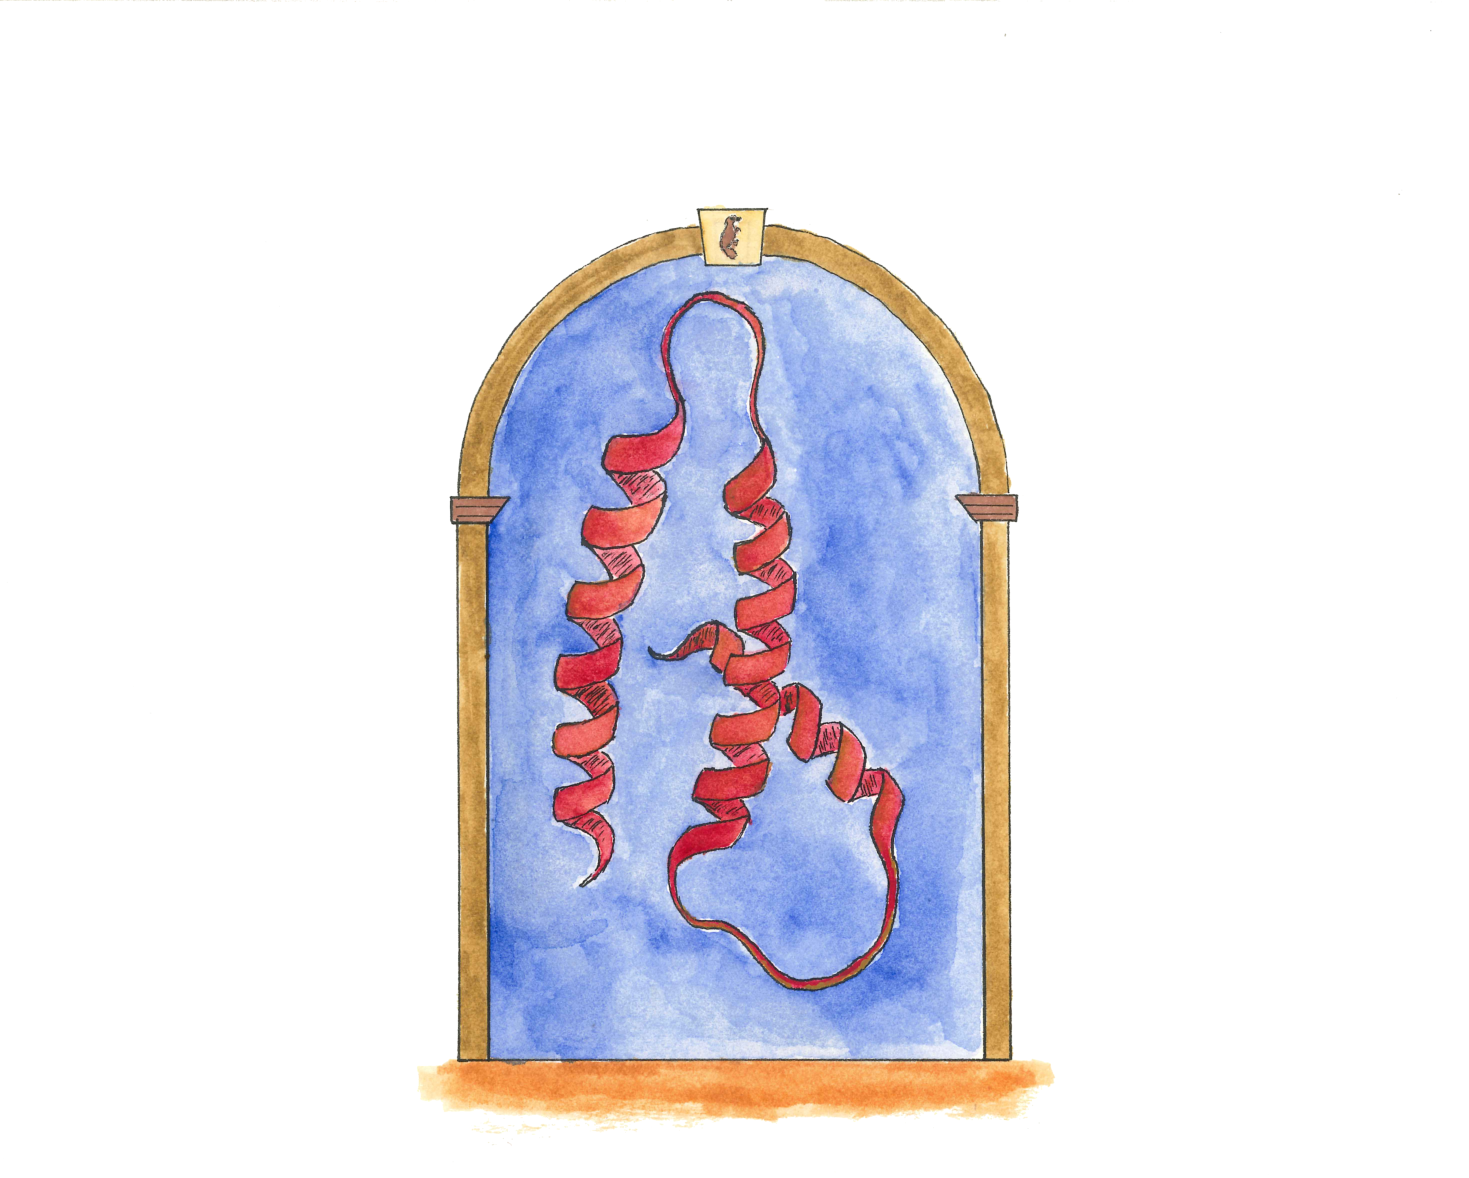
\includegraphics[trim={7cm, 0, 7cm, 0}, clip, height=0.55\pageheight]{scans/inner_cover.pdf}};
    	\if\helplines1
        	\draw[help lines,xstep=.1,ystep=.1] (0,0) grid (\N,\N);
        \fi
        \if\helplines0
        	\path[help lines,xstep=.1,ystep=.1] (0,0) grid (\N,\N);
        \fi
        
        \node[align=center, anchor=north] (en) at (0.3, 0.8) {\english{\Large Explanation of the cover}};
        
        \node[align=justify, anchor=north, below=1cm of en, text width=0.4\pagewidth] {\english{The cover depicts a protein structure under an arch, a punny reference between protein structures, and the importance of the structure of the data in deep learning. This is, incidentally, why some people call it \emph{structured learning}. The arch style is inspired by the works of Vitruvius, a throwback to the Reinessance, which matches the style of the interior of the thesis.
        
        \vspace{0.5em}
        
        \doindent The keystone depicts a tiny rampant platypus.}};
        
        \node[align=left, anchor=west] (es) at (0.1, 0.3)  {\spanish{\Large Explicación de la portada.}};
        
        
        \node[align=justify, anchor=west, text width=0.8\pagewidth] (es) at (0.1, 0.18)  {\spanish{La portada muestra la estructura de una proteína bajo un arco, un juego de palabras entre las estructuras de proteínas, y la importancia de la estructura de los datos en aprendizaje profundo. Por esta razón algunos autores lo llaman \emph{aprendizaje estructurado}.
        El estilo del arco está inspirado por los diseños de Vitruvio, una referencia al Renacimiento, que harmoniza con el estilo del interior de la tésis.
        
                \vspace{0.5em}
                
        \doindent La clave representa un ornitorrinco rampante.}};
        
    \end{scope}
\end{tikzpicture}
\end{center}

\begin{center}
\begin{tikzpicture}
    \begin{scope}[x={(current page.south east)},y={(current page.north west)}]
        \if\helplines1
        	\path[draw, help lines,xstep=.1,ystep=.1] (0,0) grid (\N, \N);
        \else
            \path[help lines,xstep=.1,ystep=.1] (0,0) grid (\N, \N);
        \fi
        \node[text width=0.4\pagewidth, align=justify, anchor= west](titleen) at (0.075, 0.5){\english{\normalsize The English text is set in \emph{IM Fell English}, a type cut by Christoffel van Dijck and Robert Granjon. In 1672, John Fell, Bishop of Oxford, bought them for the printer in Oxford.
		Nowadays the are not only the oldest surviving punches in England, but are still being used in new books.
         
        \doindent The digital incarnation was created by Igino Marini between 2000 and 2006.}};
		
		
		\node[text width=0.401\pagewidth, align=justify, anchor= west] (titlees) at (0.525, 0.5) {\spanish{\normalsize \oldstylenums El texto en español está tipografiado en una fuente grabada por  Jerónimo Antonio Gil en el siglo XVIII. Fue seleccionada para la edición de \emph{El Quijote} publicada por la Real Academia en \oldstylenums{1780}. 
		
		\doindent La versión digital, llamada \emph{Ibarra Real} fue resucitada por la Calcografía Nacional y José María Ribagorda en el año \oldstylenums{2005}.}};
    \end{scope}

\end{tikzpicture}
\end{center}

% Final page
\begin{figure}
\centering
\includegraphics[width=0.7\textwidth]{scans/back_cover.png}
\end{figure}

\end{document}
